\documentclass{mywork}
\blattnumeins

\begin{document}

\setcounter{aufgabe}{3}
\begin{aufgabe}
	\begin{enumerate}[a)]
		\item
			Splineinterpolation:
			\begin{lstlisting}[language=matlab,tabsize=4]
% Stephan Hilb, 2706616
function S = myspline (X, Y)
	n = length(X);
	H = diff(X);
	
	A = diag(2*(H(1:n-2) + H(2:n-1)));
	A = A + diag(H(2:n-2), 1) + diag(H(2:n-2), -1);

	b = (6 ./ H(2:n-1)) .* (Y(3:n) - Y(2:n-1));
	b = b - (6 ./ H(1:n-2)) .* (Y(2:n-1) - Y(1:n-2)) ;

	M(1) = 0;
	M(2:n-1) = A \ b;
	M(n) = 0;
	M = transpose(M);

	S(1,:) = (M(2:n) - M(1:n-1)) ./ (6 * H);
	S(2,:) = M(1:n-1) ./ 2;
	S(3,:) = ((Y(2:n) - Y(1:n-1)) ./ H) ...
		- (H .* (M(2:n) ./ 6 + M(1:n-1) ./ 3));
	S(4,:) = Y(1:n-1);
end
			\end{lstlisting}
		\item
			Siehe Plot
		\begin{figure*}[h]
			\centering
			\caption{Splineinterpolation zu $n\in \{4,8,16,32\}$}
			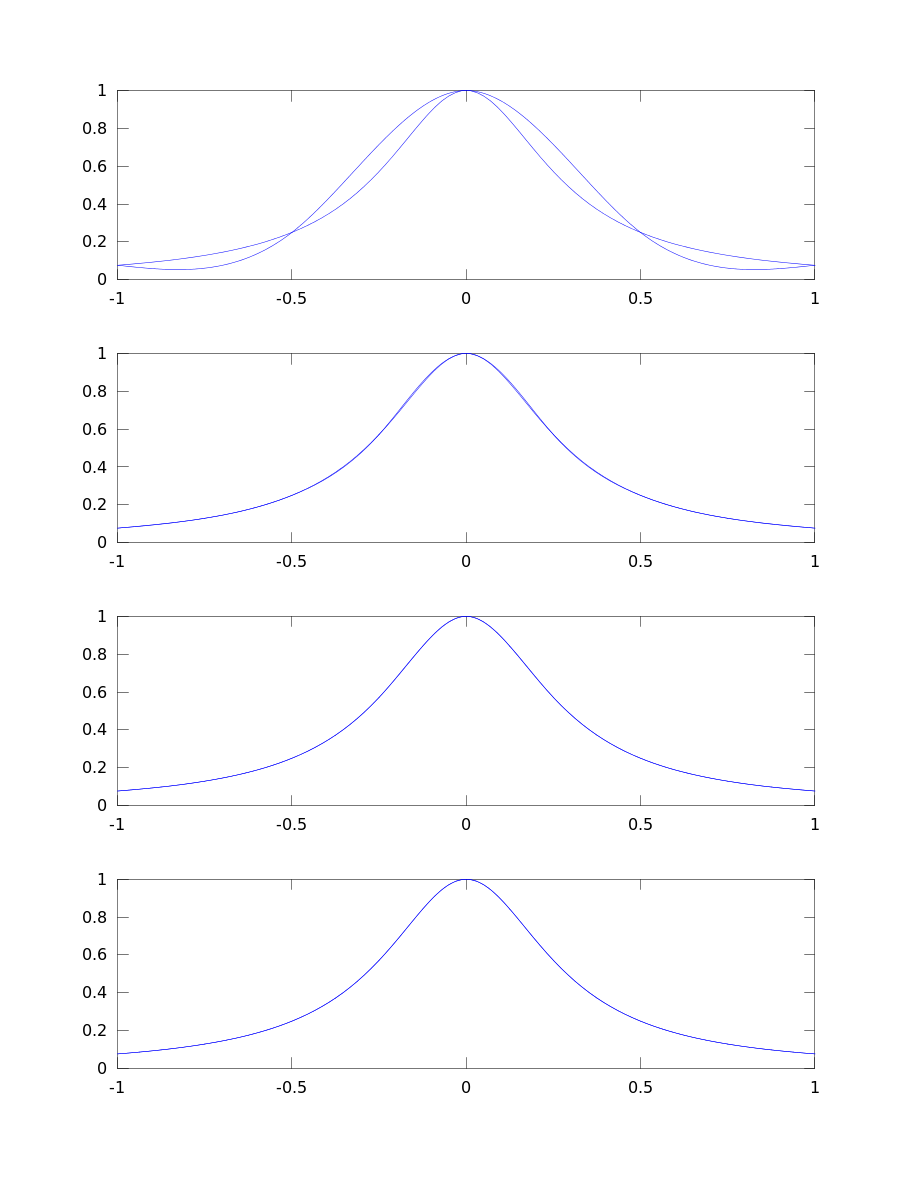
\includegraphics[scale=0.5]{num1_5_4/num1_5_4.png}
		\end{figure*}
		\item
			~

		\begin{table}[h]
			\centering
			\caption{Fehler und EOC-Werte (EOC bezogen auf die beiden Vorgänger $n$s)}
			\begin{tabular}{l|rrrr}
				$n$ & 4 & 8 & 16 & 32 \\ \hline
				Fehler & 1.4347e-01 & 1.2702e-03 & 2.1879e-03 & 1.5505e-04 \\ \hline
				EOC & & 3.9520 & 2.0830 & 3.8188
			\end{tabular}
		\end{table}
		\newpage
		\item
			\begin{lstlisting}[language=matlab,tabsize=4]
% Stephan Hilb, 2706616

a = -1;
b = 1;

N = [4,8,16,32];
clf;
for i = (1:4)
	e(i) = 0;
	n = N(i);
    subplot(4, 1, i);
	title("abc");

	X = linspace(a, b, n + 1);
	H = diff(X);
	Y = 1 ./ (1 .+ 12 * X.^2);
	S = myspline(transpose(X), transpose(Y));

	plot(linspace(a,b), 1 ./ (1 .+ 12 * linspace(a,b).^2));


	hold on;
	for j = (1:n)
		x = linspace(X(j), X(j+1));
		y = polyval(S(:,j), linspace(0, H(j)));
		plot(x, y);
		xe = (X(j):0.001:X(j+1));
		ye = 1 ./ (1 .+ 12 * xe.^2);
		se = polyval(S(:,j), (0:0.001:H(j)));
		etmp = max(abs(ye - se));
		e(i) = max(e(i), etmp);
	end
	hold off

	if i > 1
		eoc(i-1) = log(e(i-1) / e(i)) / log( (2/N(i-1)) / (2/N(i)) );
	end
end
e
eoc
			\end{lstlisting}
	\end{enumerate}
\end{aufgabe}


\end{document}
